%% Необхоимый минимум
\documentclass[a4paper,12pt]{article}



%%% Работа с русским языком
\usepackage{cmap}					% поиск в PDF
\usepackage{mathtext} 				% русские буквы в формулах
\usepackage[T2A]{fontenc}			% кодировка
\usepackage[utf8]{inputenc}			% кодировка исходного текста
\usepackage[english,russian]{babel}	% локализация и переносы



%%% Дополнительная работа с математикой
\usepackage{amsfonts,amssymb,amsthm,mathtools} % AMS
\usepackage{amsmath}
\usepackage{icomma} % "Умная" запятая: $0,2$ --- число, $0, 2$ --- перечисление

%% Номера формул
\mathtoolsset{showonlyrefs=true} % Показывать номера только у тех формул, на которые есть \eqref{} в тексте.

%% Шрифты
\usepackage{euscript}	 % Шрифт Евклид
\usepackage{mathrsfs} % Красивый матшрифт

%% Свои команды
\DeclareMathOperator{\sgn}{\mathop{sgn}}

%% Перенос знаков в формулах (по Львовскому)
\newcommand*{\hm}[1]{#1\nobreak\discretionary{}
	{\hbox{$\mathsurround=0pt #1$}}{}}

\usepackage{gensymb}
\usepackage{indentfirst}
\usepackage{lscape}

\usepackage{caption}
\captionsetup{labelsep=period}
\captionsetup{justification=centerlast}
\usepackage{subcaption}
\renewcommand{\thesubfigure}{\asbuk{subfigure}}

\usepackage{microtype}


%%% Параметры страницы: поля, колонтитулы, интерлиньяж
\usepackage{extsizes} % Возможность сделать 14-й шрифт
\usepackage{geometry} % Простой способ задавать поля
\geometry{top=20mm}
\geometry{bottom=20mm}
\geometry{left=25mm}
\geometry{right=15mm}

%\usepackage{fancyhdr} % Колонтитулы
%\pagestyle{fancy}
%\renewcommand{\headrulewidth}{0mm}  % Толщина линейки, отчеркивающей верхний колонтитул
%\lfoot{Нижний левый}
%\rfoot{Нижний правый}
%\rhead{Верхний правый}
%\chead{Верхний в центре}
%\lhead{Верхний левый}
% \cfoot{Нижний в центре} % По умолчанию здесь номер страницы

%\usepackage{setspace} % Интерлиньяж
%\onehalfspacing % Интерлиньяж 1.5
%\doublespacing % Интерлиньяж 2
%\singlespacing % Интерлиньяж 1

%%% Работа с таблицами
\usepackage{array,tabularx,tabulary,booktabs} % Дополнительная работа с таблицами
\usepackage{longtable}  % Длинные таблицы
\usepackage{multirow} % Слияние строк в таблице

%%% Работа с картинками
\usepackage{graphicx}  % Для вставки рисунков
\graphicspath{{images/}{images2/}}  % папки с картинками
\setlength\fboxsep{3pt} % Отступ рамки \fbox{} от рисунка
\setlength\fboxrule{1pt} % Толщина линий рамки \fbox{}
\usepackage{wrapfig} % Обтекание рисунков и таблиц текстом

\usepackage{lastpage} % Узнать, сколько всего страниц в документе.

\usepackage{soul} % Модификаторы начертания
\usepackage{soulutf8} % Модификаторы начертания

%\renewcommand{\familydefault}{\sfdefault} % Начертание шрифта

\usepackage{multicol} % Несколько колонок

\begin{document}
\thispagestyle{empty}
\begin{center}
	\large
	{\scshape министерство образования и науки\\российской федерации}
	\vspace{1ex}
	
	{\scshape национальный исследовательский ядерный\\университет <<мифи>>}
	\vspace {5 cm}
	
	\Large
	{\scshape \textbf{отчет}\\о проделанной работы в рамках подготовки ВКР}
\end{center}

\vspace{3cm}
%\begin{flushright}
\hfill
\parbox{0.5\linewidth}{
\textbf{Выполнил}\\студент группы С19-103 Мамлеев А.А.\\[1ex]

\textbf{Научный руководитель}\\
кандидат технических наук Куценко К.В.\\[2ex]
Оценка: 
}
%\end{flushright}

\vfill

\begin{center}
	Москва 2023
\end{center}
\newpage
\section{Введение, актуальность}
Естественная конвекция уже довольно продолжительное время исследуется как теоретическими, так и аналитическими методами. С развитием информационных технологий для решений данного класса теплофизических задач стали также активно применять численные методы. В данной работе будет рассмотрена задача оптимизации теплообмена с двух расположенных друг над другом ТВЭЛов путем выбора оптимального расстояния между ними. Данная задача имеет не только большой исследовательский интерес, но и большую практическую значимость. Путем выбора наиболее оптимальной геометрии относительного расположения теплоотдающих поверхностей можно одновременно повысить коэффициент теплоотдачи и увеличить удельное тепловыделение (тепловыделение в единице объема).

\section{Постановка задачи}
Имеются два горизонтальных ТВЭЛа одинакового диаметра $d$ и мощности, расположенных друг над другом (рис.~\ref{fig:phys_geom}). Необходимо определить, на каком расстоянии $s$ наиболее оптимально располагать верхний ТВЭЛ относительно нижнего для интенсификации теплообмена. Задача рассматривается в двухмерной геометрии. Пространство под нижним ТВЭЛОм не ограничено (бездонный сосуд), пространство справа и слева от ТВЭЛов также не ограничено (бесконечно удаленные стенки), расстояние от верхнего ТВЭЛа до верхней границы $h$ конечно. Изучение влияния данного расстояния на расчетные поля также входит в рассматриваемую задачу.

В \emph{численной постановке} ширина $W$ и высота $H$ области конечны (рис.~\ref{fig:num_geom}), их значения выбираются достаточно большими для того, чтобы минимизировать эффекты связанные с ограниченностью области решения задачи.

\subsection{Граничные условия}
Верхняя граница в физической постановке соответствует свободной поверхности жидкости. Для имитации свободной поверхности жидкости в численной модели выбрано граничное условие \emph{скольжения} для скорости. Выбор граничных условий также усложнен наличием в численной модели отсутствующих в физической постановки границ: нижней и боковых. Граничные условия на этих границах должны сделать границы <<прозрачными>>, <<свободными>>. В таблице~\ref{tab:boundary_cond} приведены граничные условия для скорости, давления и температуры. Отдельно стоит отметить условие давления на верхней границы: на ней выбрано сложное граничное условие "--- решатель автоматически подбирает величину градиента давления для того, чтобы поток вещества через поверхность был равен нулю. 
\begin{figure}[t]
\parbox[t]{0.4\linewidth}{
\centering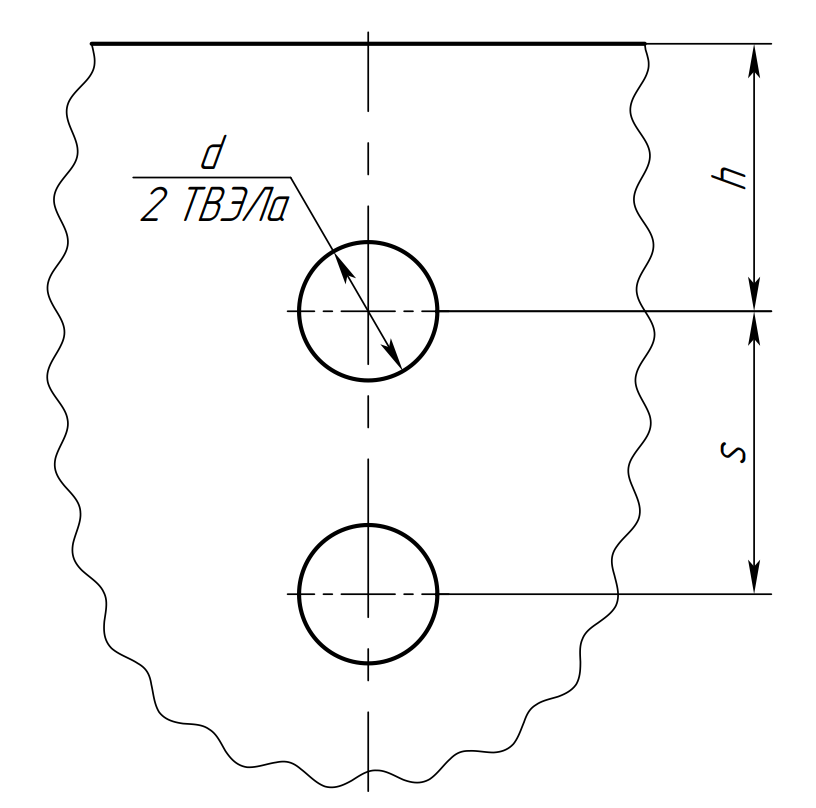
\includegraphics[width=\linewidth]{phys_geom}
\caption{Геометрия задачи} \label{fig:phys_geom}
}
\hfill
\parbox[t]{0.45\linewidth}{
\centering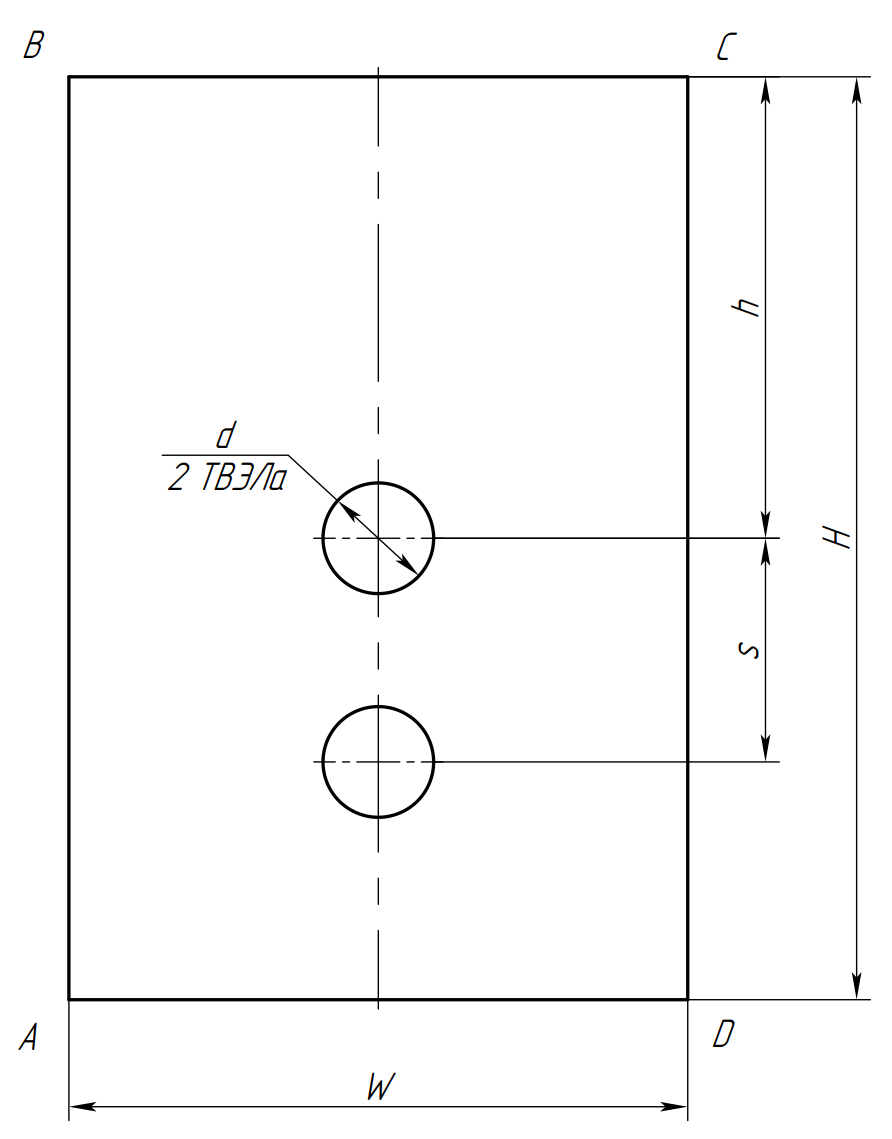
\includegraphics[width=\linewidth]{num_geom}
\caption{Геометрия для численного моделирования} \label{fig:num_geom}
}
\end{figure}

\begin{table}[h]
	\centering
	\caption{Граничные условия} \label{tab:boundary_cond}
	\begin{tabular}{|l|l|l|l|}
		\hline
		Граница (рис. \ref{fig:num_geom}) & Скорость $u$ & Температура $T$ & Давление $p = p_{абс}-\rho g z$ \\ \hline
		Поверхности ТВЭЛов &
		\begin{tabular}[c]{@{}l@{}}Первое краевое:\\  $u = 0$\end{tabular} &
		\begin{tabular}[c]{@{}l@{}}Второе краевое:\\  $-\lambda \frac{\partial T}{\partial n} = q_0$\end{tabular} &
		\begin{tabular}[c]{@{}l@{}}Второе краевое:\\ $\frac{\partial p}{\partial n} = 0$\end{tabular} \\ \hline
		Верхняя граница $BC$ &
		\begin{tabular}[c]{@{}l@{}}Первое краевое:\\  $u_n = 0$\end{tabular} &
		\begin{tabular}[c]{@{}l@{}}Первое краевое:\\ $T = T_0$\end{tabular} &
		\begin{tabular}[c]{@{}l@{}}Второе краевое:\\ $\frac{\partial p}{\partial n} = f(u)$\end{tabular} \\ \hline
		Нижняя граница $AD$ &
		\begin{tabular}[c]{@{}l@{}}Второе краевое:\\ $\frac{\partial u}{\partial n} = 0$\end{tabular} &
		\begin{tabular}[c]{@{}l@{}}Второе краевое:\\  $\frac{\partial T}{\partial n} = 0$\end{tabular} &
		\begin{tabular}[c]{@{}l@{}}Второе краевое:\\ $\frac{\partial p}{\partial n} = 0$\end{tabular} \\ \hline
		Боковые границы $AB,~CD$ &
		\begin{tabular}[c]{@{}l@{}}Второе краевое:\\ $\frac{\partial u}{\partial n} = 0$\end{tabular} &
		\begin{tabular}[c]{@{}l@{}}Второе краевое:\\  $\frac{\partial T}{\partial n} = 0$\end{tabular} &
		\begin{tabular}[c]{@{}l@{}}Второе краевое:\\ $\frac{\partial p}{\partial n} = 0$\end{tabular} \\ \hline
	\end{tabular}
\end{table}

\section{Методика решения}
Предполагается, что помещать верхний ТВЭЛ над нижним следует в той точке, где в отсутствие верхнего ТВЭЛа достигается максимум скорости восходящего потока от нижнего. Для этого решается вспомогательная задача с \emph{одним ТВЭЛом}, в остальном, геометрия и краевые условия остаются прежними. Во вспомогательной задачи исследуется профиль скорости над ТВЭЛом в зависимости от мощности энерговыделения и расстояния от верхней границы, проверяется возможность построения универсального профиля скорости.

В качестве \emph{инструмента} для построения численного решения применяется открытый некоммерческий набор решателей \emph{<<CFD OpenFOAM>>}. Для построения расчетной сетки и просмотра рассчитанных полей применяются также открытые программные продукты: \emph{<<SALOME>>} и \emph{<<ParaView>>} соответственно.

\subsection{Система уравнений}

Задача решается в приближении Буссинеска \cite{loiz}:
\begin{equation} \label{eq:bouss}
\left\{
\begin{aligned}
	\rho \left(\frac{\partial \vec{u}}{\partial t} + (\vec{u}\cdot \nabla)\vec{u}\right) &= -\nabla p + \mu \Delta \vec{u} + \rho(T) \vec{g},\\
	\frac{\partial T}{\partial t} + (\vec{u} \cdot \nabla) T &= a \Delta T, \\
	\nabla \vec{u} &= 0,
\end{aligned}
\right.
\end{equation}
где $\vec{u}$ "--- скорость течения, $T$ "--- абсолютная температура, $p$ "--- давление, $\mu$ "--- динамическая вязкость, $a$ "--- коэффициент температуропроводности, $\vec{g}$ "--- ускорение свободного падения.

Для зависимости плотности жидкости от температуры будет применяться линейная аппроксимация:
\begin{equation}
	\rho (T) = \rho_0 (1-\beta \theta), \label{eq:rho}
\end{equation}
где $\beta$ "--- коэффициент объемного расширения, $\theta = T - T_0$ "--- отклонения температуры от равновесного состояния, $\rho_0$ "--- плотность жидкости при равновесной температуре $T_0$.

Нас будет интересовать стационарное решение задачи ($\frac{\partial}{\partial t} = 0$), с учетом \eqref{eq:rho} система уравнений \eqref{eq:bouss} преобразуется к виду:
\begin{equation} \label{eq:bouss_beta}
\left\{
\begin{aligned}
	(\vec{u}\cdot \nabla)\vec{u} &= \frac{\nabla p}{\rho_0} + \nu \Delta \vec{u} - \beta \theta \vec{g}, \\
	(\vec{u}\cdot \nabla)\theta &= a \Delta \theta, \\
	\nabla \vec{u} &= 0, 
\end{aligned}
\right.
\end{equation}
где $\nu = \dfrac{\mu}{\rho_0}$ "--- кинематическая вязкость. В совокупности с граничными условиями (табл.~\ref{tab:boundary_cond}) система уравнений \eqref{eq:bouss_beta} однозначно разрешаемую краевую задачу. Для разрешения данной задачи используется решатель \emph{<<buoyantBoussinesqPimpleFoam>>} \cite{foam}.

\section{Проделанная работа}

Для параметров задачи $d = 16~мм$, $h = 0.2~м$, $H = 0.3~м$ были построены профили скоростей (проекции скорости на вертикальную ось) для плотностей энерговыделения $q = 1, 10, 100~Вт/м^2$ (рис.~\ref{fig:plot}). Параметры жидкости брались для воды при нормальном атмосферном давлении и температуре $20~\degree С$: $\lambda = 0.60~Вт/(м\cdot К)$, $\beta = 1.82\cdot 10^{-4}~К^{-1}$, $\text{Pr} = 7.02$, $\nu = 1.00\cdot 10^{-6}~м^2/с$.
\begin{figure}[h]
	\centering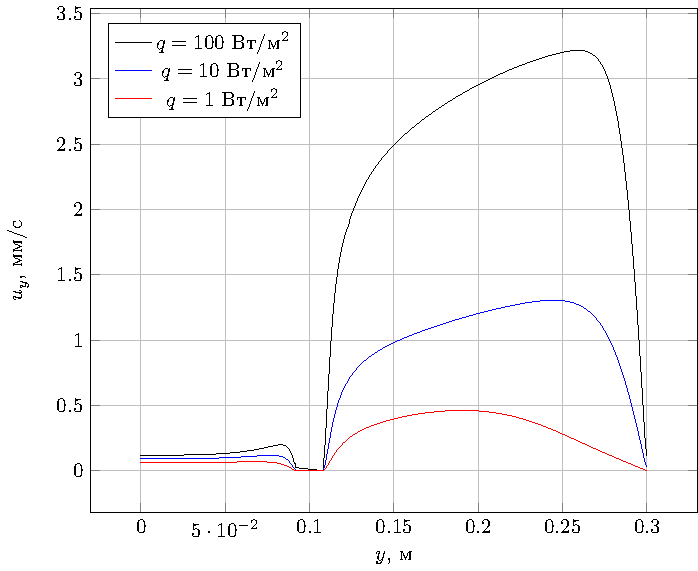
\includegraphics[width = 0.7\linewidth]{plot.pdf}
	\caption{График зависимости проекции скорости $u_y$ от вертикальной координаты $y$ на оси симметрии} \label{fig:plot}
\end{figure}

\section{Планы дальнейшей работы}

Дальнейшая работа сводится к сравнению расчета с экспериментальными данными, для чего необходимо автоматизировать расчет числа Нуссельта, а также провести расчет при параметрах, соответствующих экспериментальным. Также необходимо обезразмерить результаты численного моделирования и перейти к решению основной задачи с двумя ТВЭЛами.

\section{Заключение}

На данный этап проделано большое количество вспомогательной работы, касающейся подготовки ПО для решения поставленной задачи; были получены первые расчетные профили скорости. Достоверность результатов на данный момент остается непроверенной, что является заделом для дальнейшей работы.

\begin{thebibliography}{4}
	\bibitem{loiz}{Лойцянский Л. Г. Механика жидкости и газа. -- Учеб. для вузов. -- Изд. 6-е, перераб. и доп. --М.: Наука. Гл. ред. физ.-мат. лит., 1987. --840 с.}
	\bibitem{foam}{OpenFOAM: API Guide. URL: https://www.openfoam.com/documentation/guides/latest/api/}
	
\end{thebibliography}

\end{document}